%!TEX root = Zusammenfassung.tex

\section{Allgemeine Methoden zur Abhängigkeitsanalyse}
% ---------------------------------------------------------------------------------------------------------------------
\subsection{Konventionelle Abhängigkeitsanalyse} %2017-05-02
\label{sec:konventionelle_abhaengigkeitsanalyse}

\subsubsection{Prinzipielles Vorgehen am Beispiel (\Cref{fig:datenflussgleichungen,fig:beispielprogramm,fig:resultat})}
\label{ssub:prinzipielles_vorgehen_am_beispiel}

\begin{description}
\item[Basisfall] Synthetisierte Attribute für Zuweisungen im Parsebaum
\item[gen$\lbrack S \rbrack$] die Definitionen eines Statements $S$
\item[kill$\lbrack S \rbrack$] solche Definitionen, die von Statement $S$ überschrieben werden.
\item[zusammengesetzte Anweisungen] Verallgemeinerung von $gen[S]$ und $kill[S]$ auf zusammengesetzte Anweisungen wie Sequenz, Konditional und Schleife.
  Dafür ist eine Abschätzung notwendig:
  \begin{description}
    \item[$gen$] es \emph{könnte} generiert worden sein.
    \item[$kill$] es ist \emph{garantiert} gelöscht worden.
  \end{description}
\end{description}

Die Berechnung erfolgt entlang des Parsebaums (bottom-up) durch \emph{Datenflussgleichungen} -- oder allgemein durch Fixpunktiteration.

\begin{figure}[p]
  \centering
  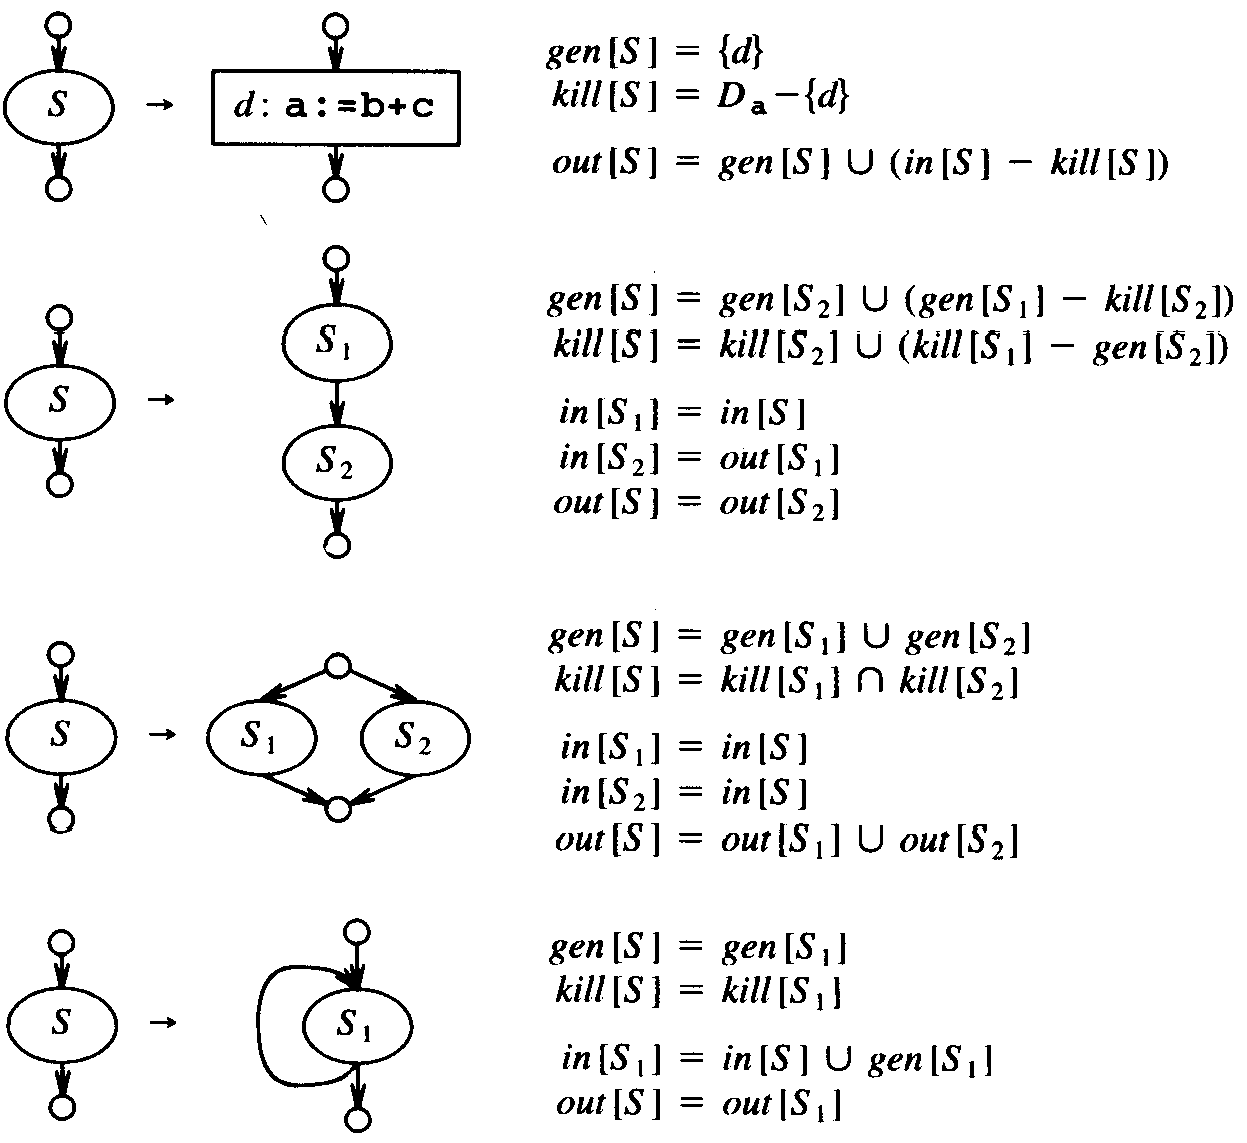
\includegraphics[scale=0.2]{images/bild1-3.png}
  % \caption{Datenflussgleichungen für \glqq erreichende Definitionen\grqq\ }
  \caption{Datenflussgleichungen für zusammengesetzte Anweisungen}
  \label{fig:datenflussgleichungen}
\end{figure}

\begin{figure}[p]
  \centering
  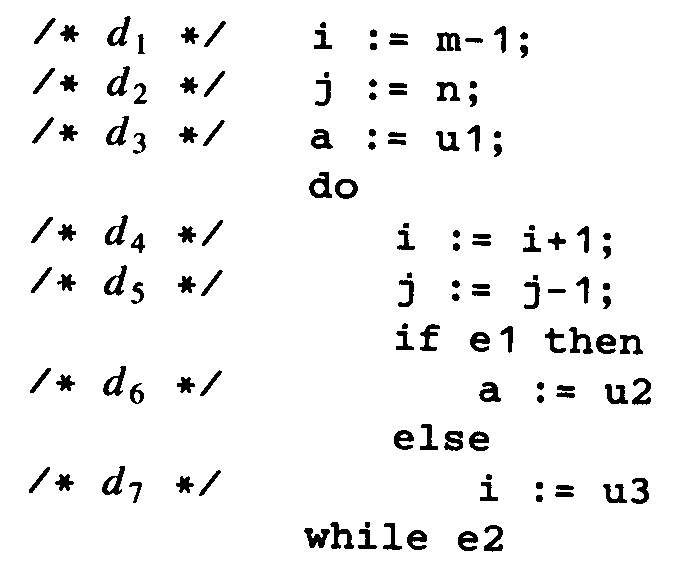
\includegraphics[scale=0.2]{images/bild3-1.png}
  \caption{Beispielprogramm}
  \label{fig:beispielprogramm}
\end{figure}

\begin{figure}[p]
  \centering
  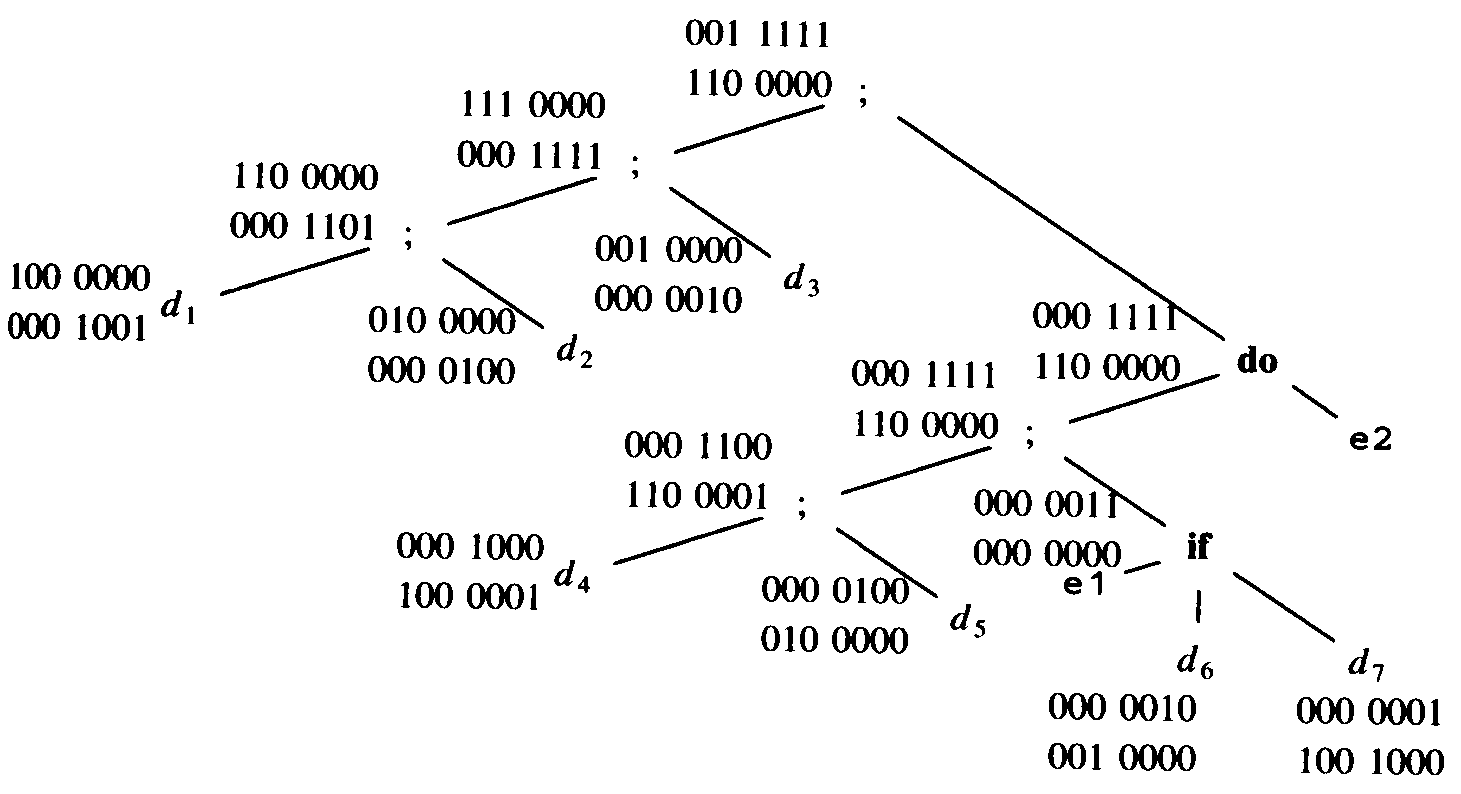
\includegraphics[scale=0.2]{images/bild2-1.png}
  \caption{Resultat der konventionellen Abhängigkeitsanalyse}
  \label{fig:resultat}
\end{figure}

\subsubsection{Nachteile dieses Verfahrens}
\label{ssub:nachteile_dieses_verfahrens}

\begin{itemize}
  \item Bitvektor-Darstellung ungeeignet für Arrays (benötigt ein bit pro Arrayzelle)
  \item teure Mengenoperationen bei sehr großen Bitvektoren
  \item Konflikte, z.\,B. für kill, nur ungenau:
    \begin{itemize}
    \item auf Variablennamen basiert (für Array ungeeignet)
    \item keine Berücksichtigung von eventuell bekannten Schleifengrenzen
    \item keine Berücksichtigung der sequentiellen Ausführungsordnung
    \end{itemize}
  \item für jedes Analyseziel ein neues Datenflussgleichungssystem von Grund auf neu berechnen
  \item im allgemeinen Fall Fixpunktiteration nötig
\end{itemize}

% ---------------------------------------------------------------------------------------------------------------------
\subsection{Polyedermodell}
\label{sec:polymod}

\subsubsection{Das ursprüngliche Modell}
\label{sec:orig-mod}

Der Schnitt von endlich vielen Halbräumen ist ein Polyeder.
Ein beschränkter Polyeder heißt Polytop.
Durch Schnitt von Hyperebenen durch Räume entstehen Halbräume.
Hyperebenen sind $n-1$-dimensionale Ebenen im $n$-dimensionalen Raum

\begin{enumerate}
\item Restriktionen:
\begin{enumerate}
\item perfekt verschachtelt
\item Schleifengrenzen: affine Ausdrücke in Strukturparametern und umgebenden
  Indizes und Maxima bzw. Minima davon (für Unter- bzw. Obergrenzen)
\item Arrayindizes affin in den Schleifenindizes und Strukturparametern
\item uniforme Abhängigkeiten
\item ein Schedule und eine Allokation für den kompletten Rumpf;
  Schedule zunächst eindimensional
%\item Schedule und Allokation linear, voneinander lin. unabhängig,
%  gemeinsam volle Dinensionalität
\end{enumerate}
%
\item Modell:
\begin{enumerate}
\item $n$-dimensionaler Schleifensatz im $n$-dimensionalen Raum (je
  Schleife eine Dimension)
\item jeder affine Ausdruck in den Schleifengrenzen definiert einen
  Halbraum
\item Polyeder: der Durchschnitt endlich vieler Halbräume
\item Polytop: beschränktes Polyeder
\item (Quell-)Indexraum ist ein Polytop
\item Abhängigkeiten durch Pfeile im Indexraum repräsentiert
\item Quellpolytop beinhaltet alle nötigen Informationen
\end{enumerate}
%
\item Raum-Zeit-Abbildung:
\begin{enumerate}
\item Schedule: Funktion, die jeder Operation einen (logischen)
  Ausführungszeitpunkt zuordnet, und dabei die durch die Abhängigkeiten
  vorgegebenen Bedingungen berücksichtigt
\item für das Modell: affine Funktion
\item graphische Bestimmung s. Beispiel der Vorlesung
\item mathematische Bestimmung: lineare Programmierung. Aufgabe:
  minimiere die affine Funktion unter der Nebenbedingung, daß ihr Wert
  für einen abhängigen Punkt größer ist als ihr Wert an dem Punkt, von
  dem er abhängt.
\item Allokation: Funktion, die jeder Operation einen (virtuellen)
  Prozessor zur Ausführung zuordnet
\item für das Modell: affine Funktion, die zum Schedule linear
  unabhängig ist (wegen der realen Maschinen und wegen des Modells
  nötig!)
\item Raum-Zeit-Abbildung: die (mehrdimensionale) affine Abbildung,
  repräsentiert durch die Transformationsmatrix, die sich aus Schedule
  und Allokation zusammensetzt, und so jeder Operation einen
  Raum-Zeit-Punkt der Ausführung zuweist. Zusätzliche Restriktion an die
  Allokation: die Raum-Zeit-Matrix muß unimodular sein (Determinante
  betragsmäßig 1)
\end{enumerate}
%
\item Transformation des Modells:
\begin{enumerate}
\item Problem: jede einzelne Dimension kann teilweise in Raum und
  teilweise in der Zeit sein
\item Ziel: Separation -- jede Dimension entweder im Raum oder in der Zeit
\item Weg: Basiswechsel = Anwendung der Raum-Zeit-Abbildung auf den
  Quell-Indexraum
\item Resultat: ``verzerrtes'' Polytop: Zielpolytop
\end{enumerate}
%
\item Zurück zum Programm:
\begin{enumerate}
\item Aufgabe: ``scanning'' der Punkte des Zielpolytops
\item parallele Schleifen für die Raumdimensionen und sequentielle
  Schleifen für die Zeitdimensionen
\item Weg: im Quell-Ungleichungssystem die Indizes durch
  ``$T^{-1}*$Zielindizes'' ersetzen und auflösen
\item abhängig von der gewünschten Reihenfolge der Zieldimensionen:
  (a)synchrones Programm
\item Quellindizes durch ``$T^{-1}*$Zielindizes'' ersetzen
\end{enumerate}
\end{enumerate}

\subsubsection{Das erweiterte Modell}
\label{sec:new-mod}

Erweiterungen:
\begin{enumerate}
\item affine Abhängigkeiten
\item stückweise affine Schedules
\item per-Statement-Schedule
\item nicht-perfekte Verschachtelung
\item nicht-unimodulare Raum-Zeit-Abbildungen
\item beliebige (z.B. nicht-invertierbare) Raum-Zeit-Abbildungen
\item beliebige Schleifentypen
\item allgemeine Array-Indizes
\end{enumerate}


\subsubsection{Abhängigkeiten in Schleifenprogrammen}
Die Abhängigkeits-Analysetechniken sind für verschachtelte
Schleifenprogramme mit Arrays als einziger Datenstruktur relativ gut
entwickelt (Skalar-Variable können dabei als null-dimensionale Arrays
interpretiert werden).

Damit ergibt sich:
\begin{enumerate}
\item Instanzen von Anweisungen sind durch die Anweisung selbst und den
  zugehörigen Iterationsvektor (Vektor der Werte aller umgebenden
  Schleifenindizes) eindeutig charakterisiert.
\item Der Indexraum einer Anweisung ist die Menge aller durch das
  Schleifenprogramm aufgezählten Indexvektoren für diese Anweisung.
\item Die sequentielle Ausführungsreihenfolge von zwei Instanzen ist
  gegeben durch die lexikographische Ordnung auf dem gemeinsamen Präfix
  ihrer Iterationsvektoren und---bei deren Gleichheit---durch die
  textuelle Reihenfolge der Anweisungen im Programmtext.
\item Speicherkonflikt liegt genau dann vor, wenn zwei Instanzen auf
  dasselbe Array zugreifen und für jede Array-Dimension auch denselben
  Index liefern. ACHTUNG: Nicht die Schleifen-Indizes, sondern die
  Array-Indizes nach dem Einsetzen der Schleifen-Indizes
  (=Iterationsvektoren) müssen übereinstimmen.
\end{enumerate}

\paragraph{Beispiel:} 3 Schleifen, 2-dim. Arrays.

\paragraph{Begriffe:}
\begin{enumerate}
\item Die Abhängigkeit geht von der \emph{Quelle} zum \emph{Ziel}.
\item Im Fall von perfekt verschachtelten Schleifen ist der
  \emph{Abhängigkeitsvektor} (oder \emph{Distanzvektor}) ist die Differenz: Ziel-Iterationsvektor minus
  Quell-Iterationsvektor. Er ist also immer lexikographisch nicht-negativ (also hinsichtlich des zeitlichen Ablaufs).
\item Eine Abhängigkeit heißt \emph{uniform}, wenn der Abhängigkeitsvektor an
  jedem Punkt des Indexraumes identisch ist.
\item Durch \emph{Richtungsvektoren}, in denen die Werte der
  Abhängigkeitsvektoren durch ihr Signum ersetzt werden, kann man selbst
  nicht-uniforme Abhängigkeiten (zu Lasten der Genauigkeit) effizient
  darstellen.
\item Eine Abhängigkeit wird von derjenigen Verschachtelungstiefe
  \emph{getragen}, deren erster Eintrag im Richtungsvektor größer als
  null ist. Ist der Richtungsvektor gleich dem Nullvektor, so heißt die
  Abhängigket \emph{schleifenunabhängig}.
\end{enumerate}
